\newpage
\section{Conception et réalisation du projet}
\label{sec:impl}

\subsection{Architecture globale du logiciel}
\paragraph{} Dans la figure \ref{fig:uml}, on a notre diagramme de classe UML avec les méthodes de chaque classes.

%\begin{figure}
%\centering
%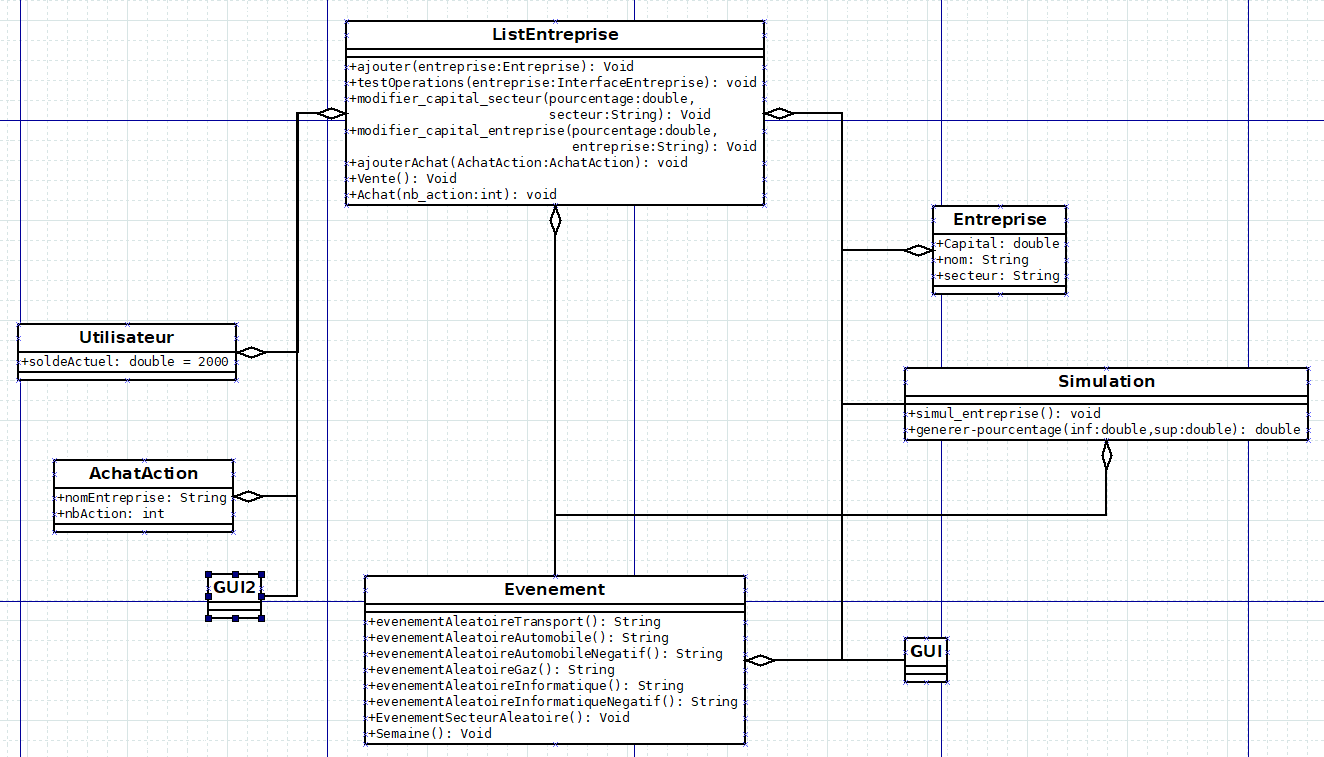
\includegraphics[width=3.5cm, height=2cm]{images/uml2.png}
%\caption{Diagramme UML}
%\label{fig:modele}
%\end{figure}

\fig{images/uml2.png}{19cm}{11.5cm}{Diagramme UML}{uml}

\subsection{Conception des classes de données}
\paragraph{} On a créer 2 classes 'objet' qui sont entreprise et utilisateur pour stocker les variables tels les capitaux, prix d'action, nom de l'entreprise, solde de l'utilisateur.

\paragraph{} Dans listEntreprise on a la création de l'arraylist contenant toute les entreprises ainsi que toutes les méthodes de manipulation d'entreprises pour modifier le capital/prix d'action ou encore faire des achats et ventes, on rappelle ses méthodes dans GUI et GUI2 ainsi que dans Evenement et simulation.
\paragraph{}Les classes simulation et Evenement contiennent les méthodes de modification de capital aléatoire par secteur ou par entreprise, les méthodes dans ces classes sont réutilisées dans GUI et GUI2.
\paragraph{}Les classes GUI et GUI2 correspondent à nos 2 fenêtres d'interface graphique, dans ses classes on rappelle les méthodes des autres classes ou on les modifie pour qu'elle soit affichables en interface graphique.
\paragraph{} 
\paragraph{} 
\subsection{Conception des traitements (processus)}
\paragraph{Le processus de notre projet consiste à chaque semaine :}
\begin{itemize}
\item De faire la simulation qui modifie entre -20 et +20 pourcent le capital de chaque entreprise.
\item Avoir un evenement aleatoire sur un secteur aléatoire.
\item Modifier le capital et le prix de l'action de chaque entreprise du secteur touché par l'evenement.
\item Achat/Vente si l'utilisateur le veut.
\end{itemize}
\paragraph{}On recommence le processus a chaque fois que l'utilisateur clique sur play


\subsection{Conception de l'IHM graphique}
\subsubsection{Première fenêtre}
\paragraph{Sur notre première fenêtre} On a la liste déroulante ou on choisis une entreprise pour soit la mettre en favori en cliquant sur "ajouter fav" ou l'afficher sur le graphique en cliquant sur "choisir entreprise". 
\paragraph{} Dans le graphique on affiche la fonction du prix d'action par rapport au temps (semaine par semaine) qui avance en cliquant play.
\paragraph{} Pour le graphique on utilise la librairie java.awt.graph et on utilise JButton pour les boutons play, ajouter fav et choisir entreprise.
\paragraph{} L'affichage des entreprises et news est fait grace a des JList.
\paragraph{}La liste des entreprises est fait avec un ListModel.

\paragraph{} Pour le graphique on a du utiliser la librairie externe JFreechart on a utiliser la commande createlineChart puis on a crée un DataSet pour stocker les valeurs a afficher dans le graphique.


%\begin{figure}
%\centering
%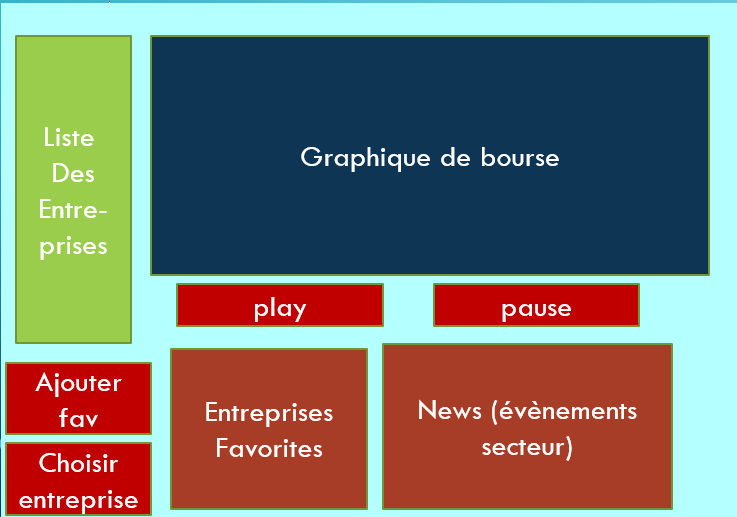
\includegraphics[width=3.5cm, height=2cm]{images/fenetre1.png}
%\caption{Première fenêtreL}
%\label{fig:modele}
%\end{figure}

\fig{images/fenetre1}{10.5cm}{7cm}{Première fenêtre}{Première fenêtre}


\paragraph{} 
\paragraph{} 
\paragraph{} 

\subsubsection{Deuxième fenêtre}
\paragraph{Sur notre deuxième fenêtre}on a crée des JList pour afficher les actions possédées et l'historique d'achat.
\paragraph{} On a ensuite une zone d'achat avec la liste deroulante des entreprises et une liste deroulante pour choisir le nombre d'action (JList) et un Jbutton pour valider l'achat d'action. 
\paragraph{} On a effectué de meme pour la partie vente.

%\begin{figure}
%\centering
%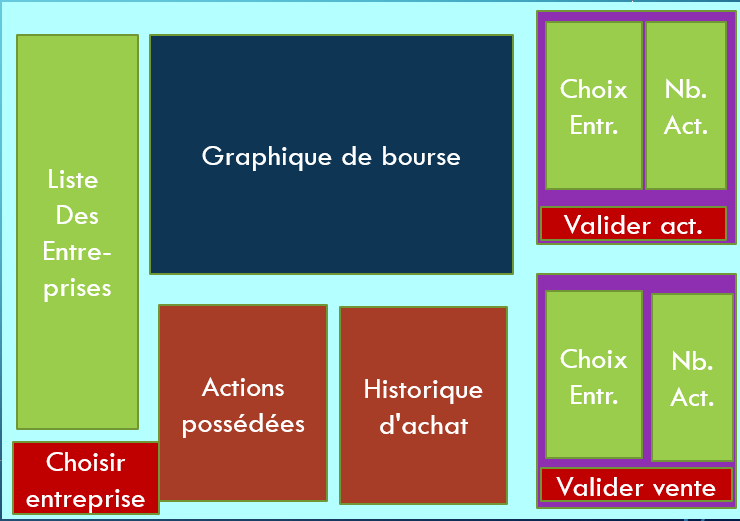
\includegraphics[width=3.5cm, height=2cm]{images/fenetre2.png}
%\caption{deuxième fenêtre}
%\label{fig:modele}
%\end{figure}

\fig{images/fenetre2.png}{10.5cm}{7cm}{deuxième fenêtre}{deuxième fenêtre}

